\pdfoutput=1

\documentclass{l4proj}

%
% put any packages here
%

\begin{document}
\title{A Front End Programming Langauge For the Glasgow Parallel Reduction Machine}
\author{Ross Meikleham}
\date{January 2015}
\maketitle

\begin{abstract}
\begin{abstract}
In the past most software was written with serial computation in mind 
and increases in processor speeds over time would in turn increase the speed 
the software ran at.
However with the rate of increase in processor speeds declining and 
manufacturers focusing on adding more processor cores this is no longer the case.
The result is that serially written software needs to be rewritten
if it wishes to take advantage of multiple processors. This project
focuses on designing a language which is familiar to most programmers
that describes the composition of serial tasks written in C++ and
can be executed in parallel. 
\end{abstract}

\end{abstract}

\educationalconsent
%
%NOTE: if you include the educationalconsent (above) and your project is graded an A then
%      it may be entered in the CS Hall of Fame
%
\tableofcontents
%==============================================================================

\chapter{Introduction}
\pagenumbering{arabic}
\chapter{Introduction}

In this section we introduce what the Glasgow Parallel Reduction machine. The aims of the project, 
and research into what Parallel Frameworks are currently available to.

\section{GPRM}

\subsection{What is the GPRM}

The Glasgow Parallel Reduction Machine is a virtual machine framework for multi-core programming using a task-based approach. It allows the programmer to structure their programs as a seperation of task-code (written as C++ classes) and communication code. 

Communication code is currently written in a language called GPIR (Glasgow Parallel Intermediate Representation). 
GPIR code controls how tasks communicate with one another and whether groups
of tasks can be evaluated sequentially or in parallel.  GPIR code is compiled down further to GPRM byte-code which is evaluated by the GPRM virtual machine.

The GPRM uses task nodes which consists of a task kernel and a task manager.

Task code is represeted as a task kernel. A task kernel is a self contained unit, typically represented as a C++ class.
To create a task kernel, the C++ class needs to be in the \textit{GPRM::Kernel::namespace}.

Communication code is represented as a task manager. A task manager "co-ordinates" communication between one or more task kernels, and
is represented as a function which can be called from a C++ program.\cite{GPRM}

\newpage

\begin{figure}[ht]
\pdfimageresolution=110
\begin{center}
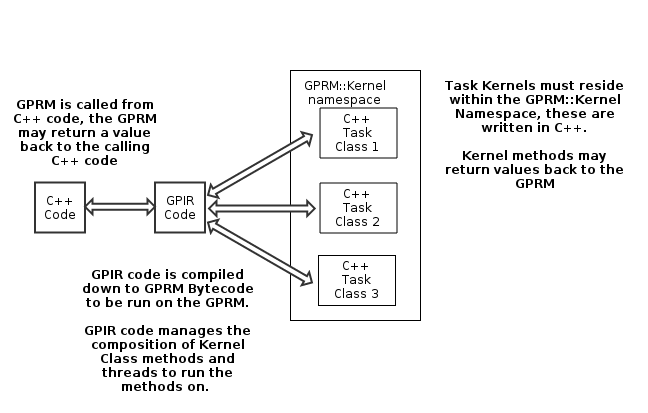
\includegraphics{graphs/gprm.png}
\caption{A simple overview of the GPRM framework}
\end{center}
\end{figure}

\subsection{The GPIR language}

The GPIR language is a purely functional S-expression based language that is evaluated in parallel by default 
with optional sequential evaluation semantics.

Tasks in GPIR are postifxed with a thread number to indicate to the GPRM runtime which thread
the task should run on. For example a simple GPIR program which adds numbers in parallel:

\begin{lstlisting}[style=myGPC]
(begin
    +[0] (+[0] '3 '2) (+[1] '4 '10)
)
\end{lstlisting}

The two nested additions are performed in parallel, with the first being mapped onto thread 0,
and the second being mapped onto thread 1. When they've both been evaluated, then the outer addition
with add the results on thread 0.

\subsubsection{Quoting}

Like in Scheme and Lisp, quoting deffers the evaluation. This is useful for performing sequential evaluation.

\begin{lstlisting}[style=myGPC]
(seq 
    '(obj.m1[0] '1)
    '(obj.m2[0] '2)
)
\end{lstlisting}

Due to the parallel evaluation of GPIR, if the expressions in the seq block wern't quoted then
they would get evaluated in parallel instead of being deffered to be evaluated by the seq function.

Also literal values don't need to be evaluated, they should be deferred and passed to tasks which is
the reason the numbers are quoted in these examples.

The GPIR language has other keywords and features but these are the ones that are important for
understanding the examples and design choices made for this project.

\section{Project Aims}

The GPIR language isn't really suitable for programming in. For one it requires the programmer to manually
manage which thread each task is allocated to. The language is also inconsistant with the C++ language used for 
the other parts of the framework (Calling code and Class Kernels). A language closer to C/C++ will be
more consistent with the entire framework.

The aim of this project is to design a C-like language which can be evaluated in parallel by default, and build
a compiler for it. The compiler should be able to compile this new language down to GPIR code. 

The language should be easy to pick up and write programs in for anyone familiar with the C/C++ languages.
To achieve this the language should be as close to C/C++ as possible 

We'll call the new language being designed " Glasgow Parallel C" or "GPC" for short.

\section{Current C/C++ Parallel Programming Models}

By researching available C/C++ parallel programming frameworks/language extensions 
we can determine possible features and design choices that may suitable for the GPC language.

\subsection{Cilk Plus}

Cilk Plus is a general purpose programming language based on C++. It extends the C++ language with features such as
parallel for loops and spawning functions in parallel using a "fork-join" model to achieve task-parallelism.

One of the main principles of the Cilk language is that abstraction is important and that the programmer should use provided constructs to expose 
the parallelism in their application. This allows the programmer to be free to focus on what the code is allowed to execute in parallel and not worry about the underlying details of manually managing threads. The run-time should then have the responsibility of scheduling the threads and dividing work between
processors.\cite{cilkfaq}. 

Cilk Plus introduces 3 new keywords on top of the C++ language\cite{cilk}: 
\begin{itemize}
    \item \textit{cilk\_for} - Parallelizing for loops, uses the exact same syntax as the standard C++ for-loop
                             with some restrictions.
    \item \textit{cilk\_spawn} - Indicate that a given function can run in parallel with the remainder
                              of the calling function. 
    \item \textit{cilk\_sync} - Wait for all spawned calls to finish.
\end{itemize}

Cilk Plus applications have "serial semantics"\cite{cilk}, this means that the results of an application run
in parallel with Cilk Plus would be exactly the same if it were run
serially (\textit{cilk\_spawn} becoming a function call, removing \textit{cilk\_sync} statements, 
and replacing \textit{cilk\_for} with ordinary for loops).

Cilk Plus makes use of pragmas to indicate to the compiler that a for loop contains data parallelism.\cite{cilkfaq}

Cilk Plus also introduces a new operator \textbf{[:]} to select array sections\cite{cilkarray}. This operator
allows for "high level" operations to be performed on arrays, and can help the compiler vectorize parts of code.

The Cilk Plus runtime makes use of "task stealing" for dynamic load balancing\cite{cilkfaq}. This 
means that if one thread is idle the scheduler can reassign work assigned to be completed by a busier thread. 
The outcome of this is that the programmer doesn't have to worry about the specifics of which threads
to map tasks to, and it can be left to the runtime itself.



\subsection{Open MP}

OpenMP (Open Multi-Processing) is a language extension available for C, C++ and Fortran which allows for shared memory multi-processing. 
This is achieved by the use of compiler directives (more specifically in C/C++ this is done through the preprocessor using pragmas). 
This allows a compiler which doesn't implement OpenMP extensions to still compile C/C++ code
and run it in a linear fashion, and serial code can be made parallel purely through the use of preprocessor
directives without modification to the actual source code.  

\subsection{Intel Thread Building Blocks}

Intell TBB (Intell Thread Building Blocks) is a portable C++ template library for task parallelism.
It contains a range of concurrent algorithms, containers, and it's own task scheduler to achieve this.

Operations are treated as tasks, and the task scheduler has the job of dynamically allocating these tasks 
to individual cores. Abstracting the specific details of allocating threads from the Programmer. 

Using templates allows for 


\section{Wool}
Wool\cite{wool} is a library which is inspired by Cilk that supports task parallel programming by introducing three forms of synchronization. (Create, Exit, and Join). It relies on tasks having low overheads. The 





\section{Project Aims}

The GPIR language isn't really suitable for programming in. For one it requires the programmer to manually
manage which thread each task is allocated to. The language is also inconsistant with the C++ language used for 
the other parts of the framework (Calling code and Class Kernels). A language closer to C/C++ will be
more consistent with the entire framework.

The aim of this project is to design a C-like language which can be evaluated in parallel by default, and build
a compiler for it. The compiler should be able to compile this new language down to GPIR code. 

The language should be easy to pick up and write programs in for anyone familiar with the C/C++ languages.
To achieve this the language should be as close to C/C++ as possible 

We'll call the new language being designed " Glasgow Parallel C" or "GPC" for short.


\section{GPRM}

\subsection{What is the GPRM}

The Glasgow Parallel Reduction Machine is a virtual machine framework for multi-core programming using a task-based approach. It allows the programmer to structure their programs as a seperation of task-code (written as C++ classes) and communication code. 

Communication code is currently written in a language called GPIR (Glasgow Parallel Intermediate Representation). 
GPIR code controls how tasks communicate with one another and whether groups
of tasks can be evaluated sequentially or in parallel.  GPIR code is compiled down further to GPRM byte-code which is evaluated by the GPRM virtual machine.

The GPRM uses task nodes which consists of a task kernel and a task manager.

Task code is represeted as a task kernel. A task kernel is a self contained unit, typically represented as a C++ class.
To create a task kernel, the C++ class needs to be in the \textit{GPRM::Kernel::namespace}.

Communication code is represented as a task manager. A task manager "co-ordinates" communication between one or more task kernels, and
is represented as a function which can be called from a C++ program.\cite{GPRM}

\newpage

\begin{figure}[ht]
\pdfimageresolution=110
\begin{center}
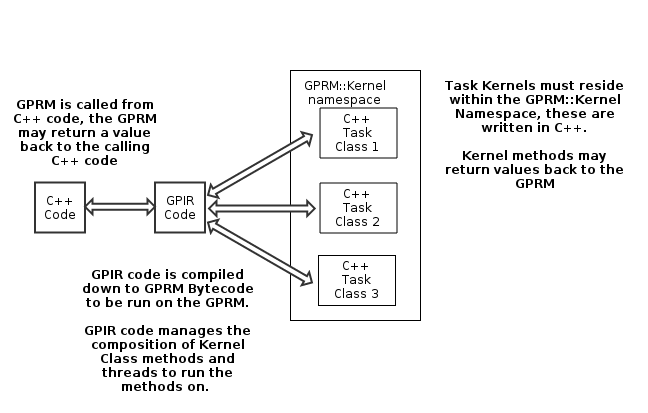
\includegraphics{graphs/gprm.png}
\caption{A simple overview of the GPRM framework}
\end{center}
\end{figure}

\subsection{The GPIR language}

The GPIR language is a purely functional S-expression based language that is evaluated in parallel by default 
with optional sequential evaluation semantics.

Tasks in GPIR are postifxed with a thread number to indicate to the GPRM runtime which thread
the task should run on. For example a simple GPIR program which adds numbers in parallel:

\begin{lstlisting}[style=myGPC]
(begin
    +[0] (+[0] '3 '2) (+[1] '4 '10)
)
\end{lstlisting}

The two nested additions are performed in parallel, with the first being mapped onto thread 0,
and the second being mapped onto thread 1. When they've both been evaluated, then the outer addition
with add the results on thread 0.

\subsubsection{Quoting}

Like in Scheme and Lisp, quoting deffers the evaluation. This is useful for performing sequential evaluation.

\begin{lstlisting}[style=myGPC]
(seq 
    '(obj.m1[0] '1)
    '(obj.m2[0] '2)
)
\end{lstlisting}

Due to the parallel evaluation of GPIR, if the expressions in the seq block wern't quoted then
they would get evaluated in parallel instead of being deffered to be evaluated by the seq function.

Also literal values don't need to be evaluated, they should be deferred and passed to tasks which is
the reason the numbers are quoted in these examples.

The GPIR language has other keywords and features but these are the ones that are important for
understanding the examples and design choices made for this project.

%The first page, abstract and table of contents are numbered using Roman numerals. From now on pages are numbered
%using Arabic numerals. Therefore, immediately after the first call to $\backslash$chapter we need the call
%$\backslash$pagenumbering$\{$arabic$\}$ and this should be called once only in the document. 

%The first Chapter should then be on page 1. You are allowed 50 pages for a 30 credit project and 35 pages for a 
%20 credit report. This includes everything up to but excluding the appendices and bibliograph, i.e. this is a limit on
%the body of the report.

%You are not allowed to alter text size (it is currently 11pt) neither are you allowed to alter the margins.

%Note that in this example, and some of the others, you need to execute the following commands the first time you process the files.
%Multiple calls to pdflatex are required to resolve references to labels and citations. The file bib.bib is the bibliography file.



%\begin{verbatim}

%            > pdflatex example0
%            > bibtex example0
%            > pdflatex example0
%            > pdflatex example0

%\end{verbatim}


%\section{First Section in Chapter}
%The quick brown fox jumped over the lazy dog.
%The quick brown fox jumped over the lazy dog \cite{DIMACS}.
%The quick brown fox jumped over the lazy dog.

%\subsection{A subsection}
%The quick brown fox jumped over the lazy dog.

%The quick brown fox \cite{fahle} jumped over the lazy dog.

%\chapter{The Fox and Dog}
%The quick brown fox jumped over the lazy dog.

%\section{The Fox Jumps Over}
%The quick brown fox jumped over the lazy dog.


%\vspace{-7mm}
%\begin{figure}
%\centering
%\includegraphics[height=9.2cm,width=13.2cm]{uroboros.pdf}
%\vspace{-30mm}
%\caption{An alternative hierarchy of the algorithms.}
%\label{uroborus}
%\end{figure}

%The quick brown fox jumped over the lazy dog.
%The quick brown fox jumped over \cite{ckt} the lazy dog.
%The quick brown fox jumped over the lazy dog.

%\section{The Lazy Dog}
%The quick brown fox jumped over the lazy dog.

%The quick brown fox jumped over the lazy dog.

%%%%%%%%%%%%%%%%
%              %
%  APPENDICES  %
%              %
%%%%%%%%%%%%%%%%
\begin{appendices}


%\chapter{Generating Random Graphs}
%\label{sec:randomGraph}
%We generate Erd\'{o}s-R\"{e}nyi random graphs $G(n,p)$ where $n$ is the number of vertices and
%each edge is included in the graph with probability $p$ independent from every other edge. It produces
%a random graph in DIMACS format with vertices numbered 1 to $n$ inclusive. It can be run from the command line as follows to produce 
%a clq file
\end{appendices}

%%%%%%%%%%%%%%%%%%%%
%   BIBLIOGRAPHY   %
%%%%%%%%%%%%%%%%%%%%

\bibliographystyle{plain}
\bibliography{bib}

\end{document}
